% =====================================================================
%  EPD-SDIA-4112 -- Statistique Bayésienne -- Master 1 SDIA
%  CHAPITRE 4 : Comparaison de modèles et décision   (50 slides, 8 h)
%  Fichier de frames : aucune dépendance à \title (build maître + build seul)
% =====================================================================
\section{Chapitre 4 --- Comparaison et décision}
\chapterslide{Chapitre 4}{Comparaison de modèles et décision}{8 h --- 5 sections --- 50 slides}{%
\textbf{Objectifs} --- quantifier la preuve par un facteur de Bayes et une échelle de
référence ; comparer des modèles hors échantillon (WAIC, LOO) ; choisir une décision qui
minimise le risque a posteriori ; conduire un A/B test sans gonfler le risque ; repérer
les pièges du BF avec un prior vague et du modèle « vrai ».}

% ---------------------------------------------------------------- 1
\begin{frame}{Objectifs pédagogiques du chapitre}
\begin{columns}[t]
\begin{column}{0.48\textwidth}
\begin{kbox}[Savoirs]
\begin{itemize}
  \item Définir le facteur de Bayes et l'interpréter en cotes
  \item Lire l'échelle de Jeffreys sans la surinterpréter
  \item Distinguer le log-score prédictif, le DIC, le WAIC et le LOO
  \item Énoncer la règle de décision qui minimise une perte a posteriori
  \item Historique : le paramètre $\theta$ est fixe (fréquentiste) contre $\theta$ aléatoire (bayésien)
\end{itemize}
\end{kbox}
\end{column}
\begin{column}{0.48\textwidth}
\begin{abox}[Savoir-faire évalués]
\begin{itemize}
  \item Calculer un $BF$ par échantillonnage et par Savage--Dickey
  \item Produire un tableau \py{az.compare()} exploitable
  \item Dériver un seuil de décision à partir d'un rapport de coûts
  \item Construire un intervalle de décision (ROPE) à trois issues
  \item Critiquer un prior (largeur, justification, sensibilité)
\end{itemize}
\end{abox}
\end{column}
\end{columns}
\vspace{1mm}
\begin{tcolorbox}[colback=byLight,colframe=byGrey!50,arc=2mm,width=.95\textwidth]
\centering\small
\textbf{Idée directrice} --- au chapitre 3 on estimait un modèle ; ici on
\textbf{compare des modèles} et on \textbf{transforme une croyance en action}
(accepter, rejeter, traiter, déployer).
\end{tcolorbox}
\end{frame}

% ---------------------------------------------------------------- 2
\begin{frame}{Plan du chapitre 4 (8 h)}
\begin{enumerate}
  \item[4.1] \textbf{Facteur de Bayes} \hfill \textit{slides 5--17}
  \item[4.2] \textbf{Critères hors échantillon} \hfill \textit{slides 18--27}
  \item[4.3] \textbf{Décision bayésienne} \hfill \textit{slides 28--38}
  \item[4.4] \textbf{A/B testing} \hfill \textit{slides 39--46}
  \item[4.5] \textbf{Synthèse, pièges et quiz} \hfill \textit{slides 47--50}
\end{enumerate}
\vspace{2mm}
\begin{tabular}{@{}lrrr@{}}
\toprule
\textbf{Volume} & \textbf{Cours magistral} & \textbf{TD} & \textbf{TP machine} \\
\midrule
8 h & 4 h 30 & 1 h 30 & 2 h \\
\bottomrule
\end{tabular}
\vspace{2mm}
\begin{tcolorbox}[colback=byPurple!6,colframe=byPurple,arc=2mm,width=.95\textwidth]
\small\centering
\textbf{Prérequis mobilisés} : posterior du chapitre 2, HDI et prédictive du chapitre 3,
\py{pymc} et \py{arviz} du chapitre 1, dérivation élémentaire.
\end{tcolorbox}
\end{frame}

% ---------------------------------------------------------------- 3
\begin{frame}{Deux questions que le chapitre 3 laissait ouvertes}
\begin{columns}[t]
\begin{column}{0.47\textwidth}
\begin{ebox}[Question 1 --- le modèle est-il bon ?]
On a estimé $\theta$. Mais \\
est-ce que le modèle $M_1$ (une seule probabilité
pour huit équipes) décrit vraiment les données, comparé à $M_2$
(huit probabilités) ou à $M_3$ (hiérarchique) ?
\vspace{1mm}
\footnotesize Un posterior net ne protège pas d'un modèle faux :
il donne une réponse précise à la mauvaise question.
\end{ebox}
\end{column}
\begin{column}{0.47\textwidth}
\begin{ebox}[Question 2 --- que faire ?]
Un test de dépistage revient positif. Faut-il traiter ? \\
Un bouton B convertit mieux que A sur 2\,000 visites.
Faut-il le déployer à 200\,000 utilisateurs ?
\vspace{1mm}
\footnotesize L'estimation ne décide pas : il faut une
\textbf{fonction de perte} et une règle.
\end{ebox}
\end{column}
\end{columns}
\vspace{1mm}
\begin{kbox}[Les trois réponses du chapitre 4]
\begin{itemize}
  \item \textbf{Facteur de Bayes} : combien de fois les données sont plus plausibles sous $H_0$ que sous $H_1$ ?
  \item \textbf{Critères hors échantillon} : quel modèle prédit le mieux une observation nouvelle ?
  \item \textbf{Décision} : quelle action minimise la perte moyenne a posteriori ?
\end{itemize}
\end{kbox}
\end{frame}

% ---------------------------------------------------------------- 4
% [suite]
\begin{frame}{4.1 Le facteur de Bayes : définition}
% [rogna]
\small
\begin{kbox}[Définition]
Pour deux modèles $M_0$ et $M_1$ munis de leurs priors $\pi_0(\theta_0)$ et $\pi_1(\theta_1)$,
\[
BF_{01} \;=\; \frac{p(y \given M_0)}{p(y \given M_1)}
\;=\; \frac{\displaystyle\int p(y \given \theta_0)\, \pi_0(\theta_0)\,\mathrm{d}\theta_0}
{\displaystyle\int p(y \given \theta_1)\, \pi_1(\theta_1)\,\mathrm{d}\theta_1}
\;=\; \frac{m_0(y)}{m_1(y)} .
\]
$m_k(y)$ est la \textbf{vraisemblance marginale} (ou \textit{évidence}) du modèle $M_k$.
\end{kbox}
\vspace{1mm}
\end{frame}

% [suite]
\begin{frame}{4.1 Le facteur de Bayes : définition (suite)}
\begin{columns}[t]
\begin{column}{0.52\textwidth}
\begin{ebox}[Lecture en cotes]
Les données transforment les cotes a priori en cotes a posteriori :
\[
\underbrace{\frac{P(M_0 \given y)}{P(M_1 \given y)}}_{\text{cotes post.}}
=\underbrace{BF_{01}}_{\text{facteur de Bayes}}\times
\underbrace{\frac{P(M_0)}{P(M_1)}}_{\text{cotes priors}}
\]
Rapport \textbf{multiplicatif}, comme un rapport de cotes en paris.
\end{ebox}
\end{column}
\begin{column}{0.44\textwidth}
\begin{kbox}[Trois propriétés]
\begin{itemize}
  \item \textbf{Symétrie} : $BF_{10} = 1/BF_{01}$
  \item \textbf{Stabilité} : $BF_{01}$ ne dépend pas du plan d'échantillonnage
        (loi de vraisemblance) ni du fait qu'on ait regardé une fois ou dix fois
  \item \textbf{Sensibilité} : $BF_{01}$ \emph{dépend} du prior choisi sous $H_1$
\end{itemize}
\end{kbox}
\end{column}
\end{columns}
\end{frame}

% ---------------------------------------------------------------- 5
% [rogna]
% [rogna]
% [rogna]
% [split]
\begin{frame}{Un rapport de vraisemblances, pas une aire de recouvrement}
\begin{center}
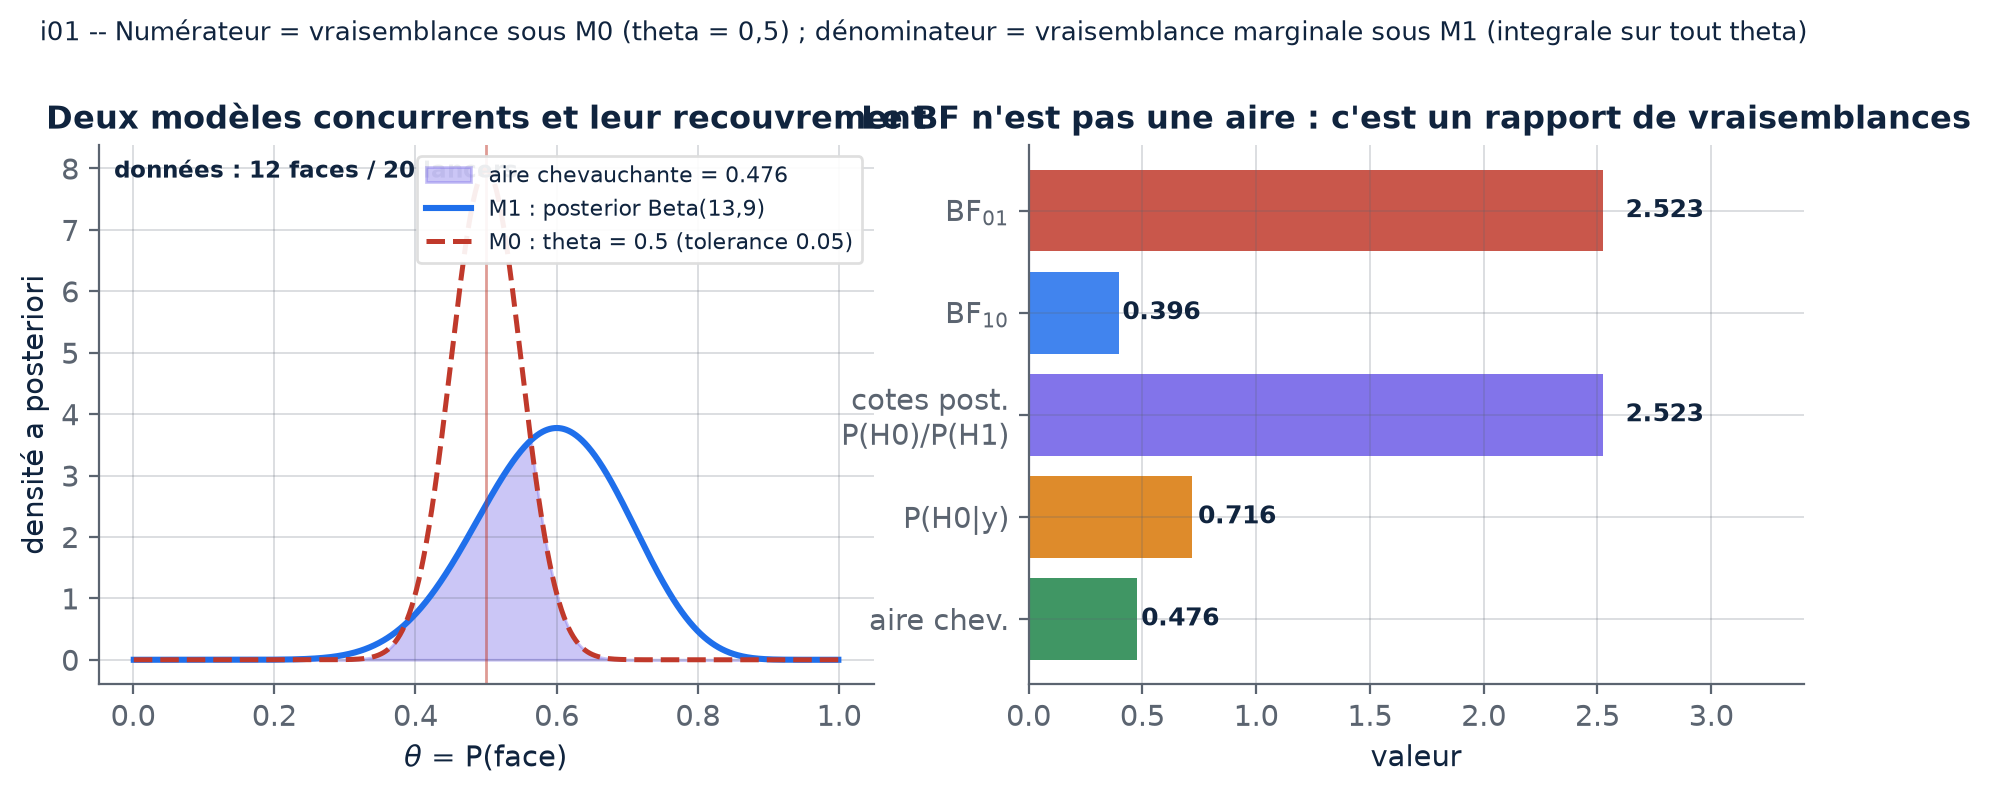
\includegraphics[width=.86\textwidth]{i01_bf_posteriors.png}
\end{center}
\end{frame}

% [split]
\begin{frame}{Un rapport de vraisemblances, pas une aire de recouvrement}

\vspace{-1mm}
\begin{columns}[t]
\begin{column}{0.54\textwidth}
\begin{ebox}[Données --- 12 faces sur 20 lancers (script \file{src/fig\_ch4.py}, exécuté)]
\begin{itemize}
  \item $M_0$ : $\theta = 0{,}5$ exactement ; $M_1$ : $\theta \sim \mathrm{Beta}(1,1)$,
        posterior $\mathrm{Beta}(13,9)$
  \item $BF_{01} = 2{,}523$, $BF_{10} = 0{,}396$ ; cotes postérieures
        (prior 1/2\,--\,1/2) $= 2{,}523$, d'où $P(M_0 \given y) = 0{,}716$
\end{itemize}
\end{ebox}
\end{column}
\begin{column}{0.42\textwidth}
\begin{wbox}[Le piège visuel]
Le recouvrement vaut $0{,}48$ et le $BF$ vaut $2{,}52$ : \textbf{aucun rapport}.
L'aire chevauchante dépend d'une tolérance arbitraire ; le rapport de vraisemblances, non.
{\footnotesize L'aire mesure une \emph{ressemblance de formes} ; le $BF$ mesure
\emph{combien de fois la donnée est plus probable}.}
\end{wbox}
\end{column}
\end{columns}
\end{frame}

% ---------------------------------------------------------------- 6
% [suite]
\begin{frame}[fragile]{Calculer un $BF$ par échantillonnage (Monte-Carlo)}
% [rogna]
\footnotesize
\begin{columns}[t]
\begin{column}{0.53\textwidth}
\begin{codebox}[Monte-Carlo depuis le prior]
\begin{lstlisting}[style=py]
import numpy as np
from math import comb, log
from scipy import special          # betaln

y, n, prior = 12, 20, (1.0, 1.0)

# 1) chemin exact : vraisemblance marginale Beta-Binomiale
lg_m0 = log(comb(n, y)) + n * np.log(0.5)
lg_m1 = (log(comb(n, y))
         + special.betaln(prior[0]+y, prior[1]+n-y)
         - special.betaln(*prior))
bf01_exact = np.exp(lg_m0 - lg_m1)          # 2.5228

# 2) chemin Monte-Carlo : BF10 = E_prior[ p(y|theta)/p(y|theta0) ]
rng  = np.random.default_rng(4112)
th   = rng.random(400_000)                  # theta ~ Beta(1,1)
ratio = (th/0.5)**y * ((1-th)/0.5)**(n-y)
bf10_mc = ratio.mean()                      # 0.39705 +/- 0.00082
bf01_mc = 1 / bf10_mc                       # 2.5185  (err. rel. 0.17 %)
\end{lstlisting}
\end{codebox}
\end{column}
\begin{column}{0.43\textwidth}
\begin{solbox}[Résultat vérifié]
Trois chemins, un seul nombre :
\begin{itemize}
  \item marginale exacte : $BF_{01} = 2{,}5228$
  \item Savage--Dickey : $2{,}5228$ (erreur relative $4\cdot10^{-16}$)
  \item Monte-Carlo (400\,000 tirages) : $2{,}5185 \pm 0{,}0052$
\end{itemize}
\vspace{1mm}
\footnotesize L'estimateur $\widehat{BF}_{10} = \frac1N\sum_i \frac{p(y \given \theta_i)}{p(y \given \theta_0)}$
n'est \emph{pas} un simple rapport de deux vraisemblances : il faut intégrer sur tout
le prior. C'est la différence structurelle avec un rapport de vraisemblance maximal.
\end{solbox}
\end{column}
\end{columns}
\end{frame}

% [suite]
\begin{frame}{Calculer un $BF$ par échantillonnage (Monte-Carlo) (suite)}
\begin{kbox}[Quand c'est instable]
Si le prior $H_1$ est très large devant la région où la vraisemblance vit, l'estimateur
Monte-Carlo a une variance énorme : on préfère alors l'intégration sur grille
(chapitre 5) ou l'échantillonnage d'importance (\py{az.loo}, \py{bridgesampling}).
\end{kbox}

\end{frame}

% ---------------------------------------------------------------- 7
\begin{frame}{Savage--Dickey : le $BF$ d'un point nul sans intégrale}
\begin{columns}[t]
\begin{column}{0.50\textwidth}
\begin{kbox}[Théorème de Savage--Dickey]
Si $H_0$ est un \textbf{point} de $H_1$ ($\theta = \theta_0$ contre $\theta \neq \theta_0$) et si
le prior $\pi_1$ est continu en $\theta_0$, alors l'évidence se lit sur le posterior :
\[
BF_{01} \;=\; \frac{\pi_1(\theta_0 \given y)}{\pi_1(\theta_0)}
\]
Un rapport de \emph{densités} au point nul, pas une intégrale sur l'espace des paramètres.
\end{kbox}
\begin{ebox}[Intuition]
Les données font \textbf{monter} la densité au point nul si $H_0$ est plausible.
$BF_{01} > 1 \iff$ la densité postérieure au point nul dépasse la densité a priori.
\end{ebox}
\end{column}
\begin{column}{0.46\textwidth}
\begin{center}
\begin{figbox}
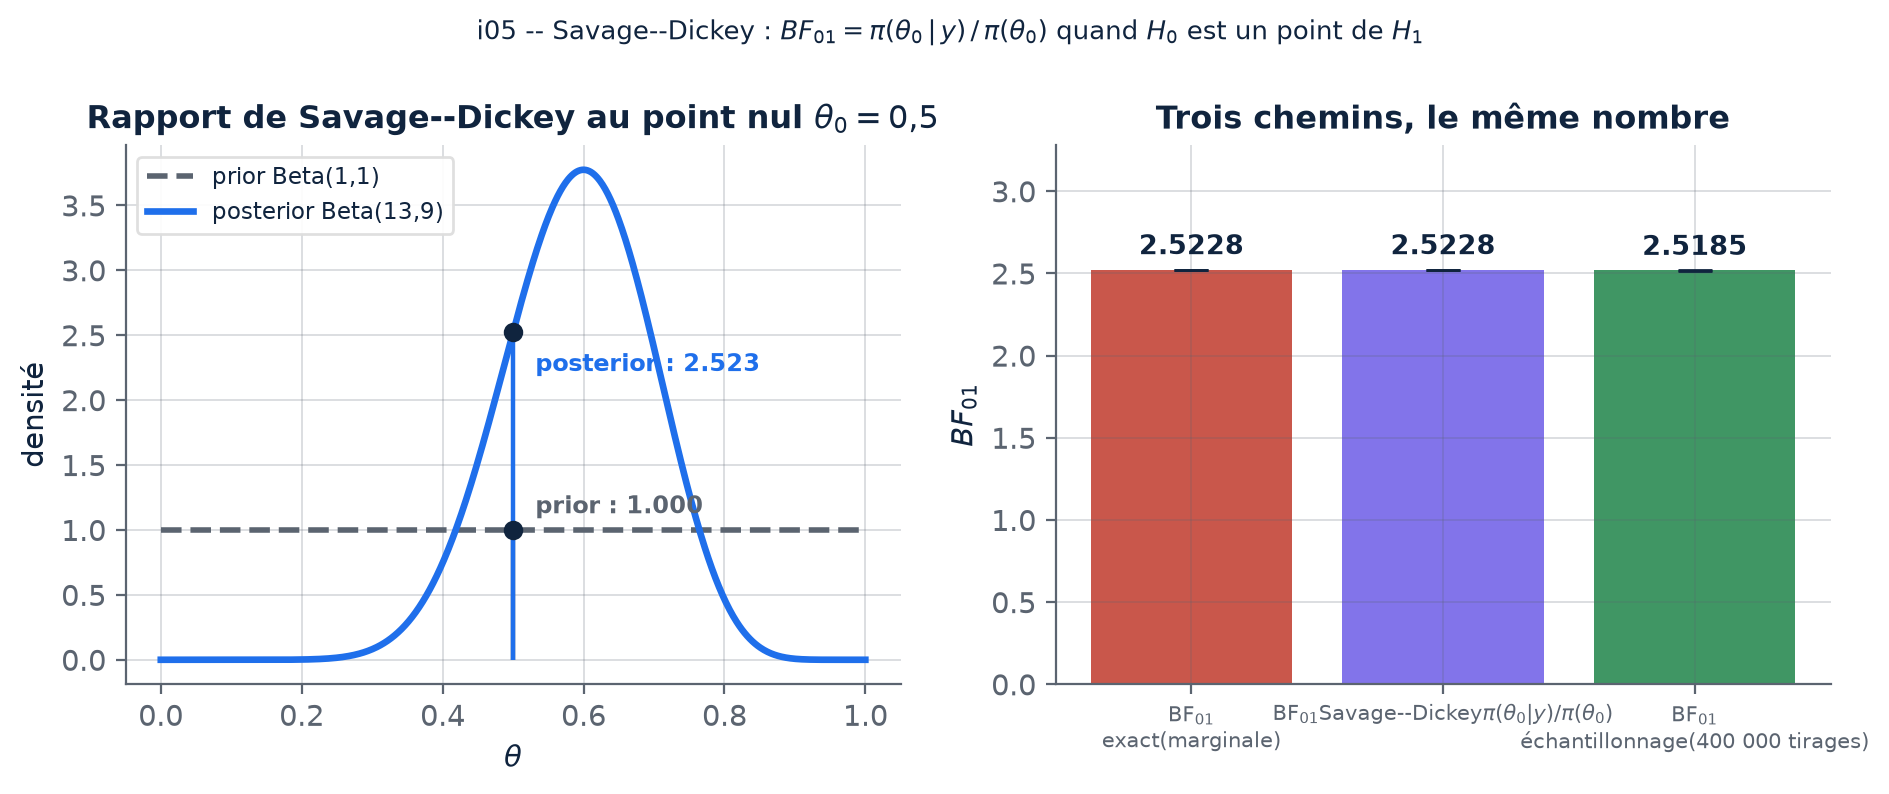
\includegraphics[width=\textwidth]{i05_savage_dickey.png}
\end{figbox}
\end{center}
\begin{solbox}[Vérifié numériquement]
$\pi(0{,}5) = 1{,}0000$ ; $\pi(0{,}5 \given y) = 2{,}5228$ ; $BF_{01} = 2{,}5228$ \\
Monte-Carlo 400\,000 tirages : $2{,}5185 \pm 0{,}0052$ (écart relatif $0{,}17\,\%$).
\end{solbox}
\end{column}
\end{columns}
\end{frame}

% ---------------------------------------------------------------- 8
\begin{frame}{L'échelle de Jeffreys : un vocabulaire, pas une loi}
\begin{center}
\small
\begin{tabular}{@{}p{2.9cm}rrp{6.0cm}@{}}
\toprule
\textbf{Interprétation} & $\log_{10} BF_{01}$ & $BF_{01}$ & \textbf{Usage en TD} \\
\midrule
Anecdotique   & $\vert\log_{10} BF\vert < 0{,}5$ & $< 3{,}2$    & ne rien conclure, collecter plus de données \\
Substantiel   & $0{,}5 \le \log_{10} BF < 1$    & $3{,}2$ à $10$  & présomption seulement \\
Fort          & $1 \le \log_{10} BF < 2$        & $10$ à $100$    & conclusion solide dans le rapport \\
Très fort     & $2 \le \log_{10} BF < 3$        & $100$ à $1\,000$ & conclusion robuste, peu de débat \\
Décisif       & $\log_{10} BF \ge 3$            & $\ge 1\,000$    & basculer la décision, publier \\
\bottomrule
\end{tabular}
\end{center}
\vspace{1mm}
\begin{columns}[t]
\begin{column}{0.47\textwidth}
\begin{kbox}[Ce que l'échelle est]
Une \textbf{convention de lecture} proposée par Jeffreys (1961), reprise par Kass et Raftery (1995).
Elle aide à verbaliser ; elle ne remplace pas un calcul de perte.
\end{kbox}
\end{column}
\begin{column}{0.49\textwidth}
\begin{wbox}[Ce que l'échelle n'est pas]
\begin{itemize}
  \item Ce n'est \textbf{pas} un seuil de significativité : $BF_{01} = 3{,}2$ n'est ni
        « significatif » ni « non significatif ».
  \item Le même $BF$ n'a pas la même importance selon l'enjeu :
        $BF_{01} = 10$ suffit pour un bouton web, jamais pour un essai clinique.
  \item Le facteur $BF_{01}$ n'est pas une probabilité : la probabilité postérieure
        exige des cotes a priori explicites.
\end{itemize}
\end{wbox}
\end{column}
\end{columns}
\end{frame}

% ---------------------------------------------------------------- 9
% [rogna]
% [rogna]
% [rogna]
% [split]
\begin{frame}{Le $BF$ s'accumule : la preuve croît linéairement en $n$}
\begin{center}
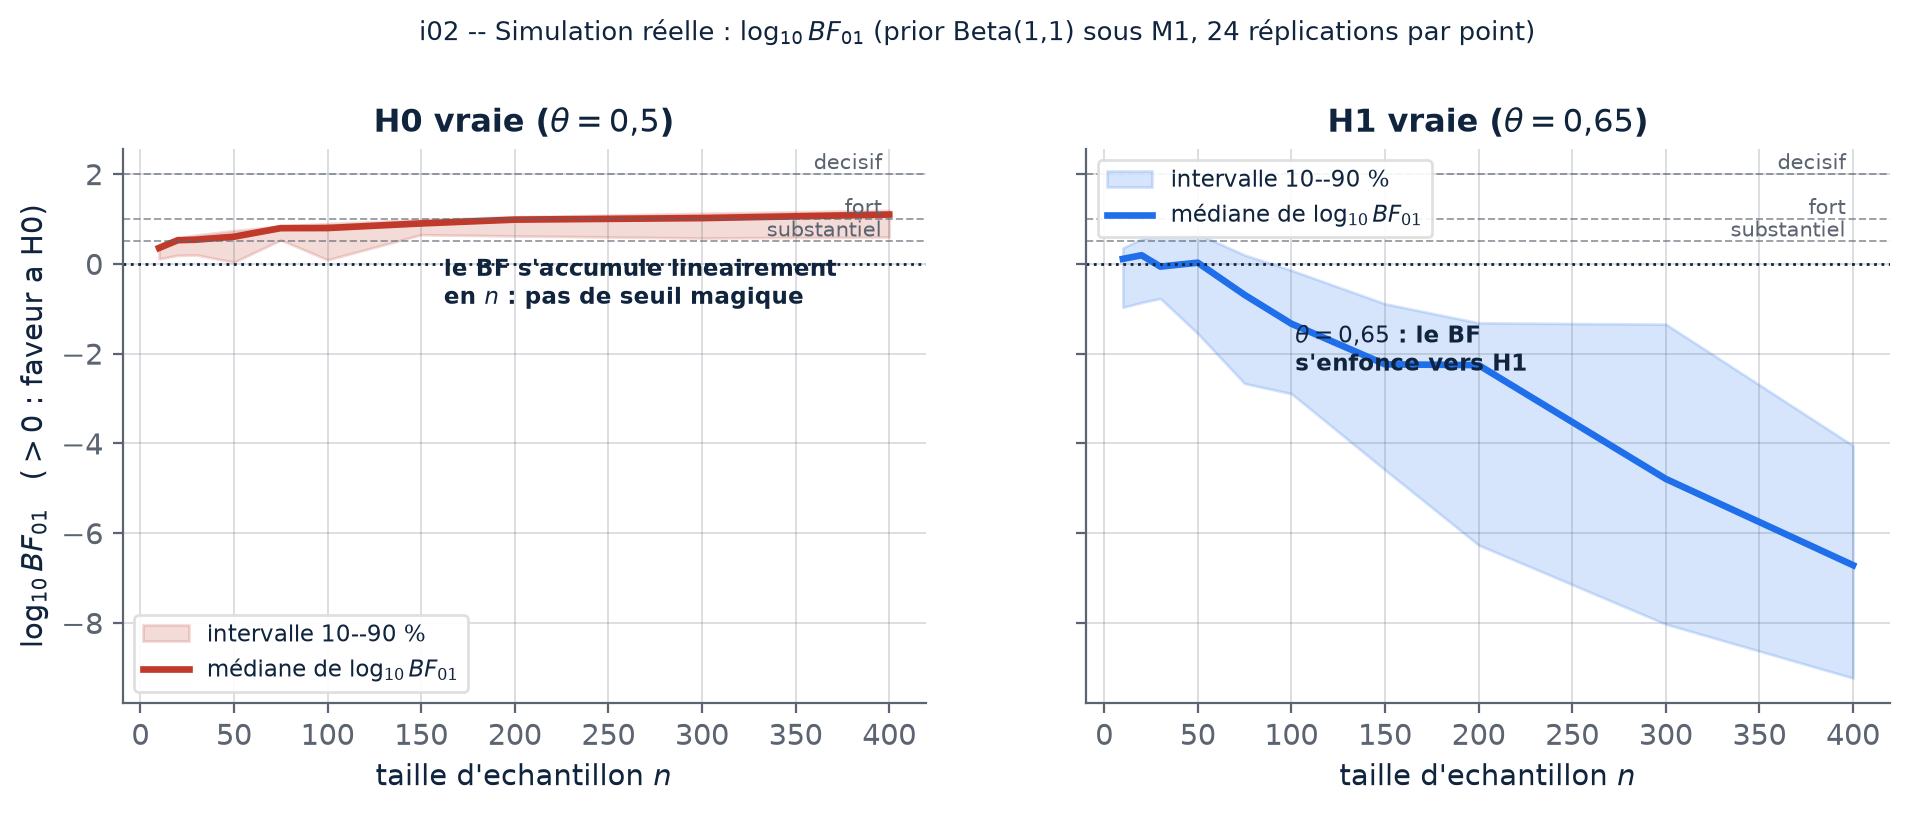
\includegraphics[width=.86\textwidth]{i02_bf_vs_n.png}
\end{center}
\end{frame}

% [split]
\begin{frame}{Le $BF$ s'accumule : la preuve croît linéairement en $n$}

\vspace{-1mm}
\begin{columns}[t]
\begin{column}{0.55\textwidth}
\begin{ebox}[Simulation réelle --- 24 réplications par point (\file{src/fig\_ch4.py})]
\begin{itemize}
  \item Sous $H_0$ vraie ($\theta = 0{,}5$) : $\log_{10} BF_{01}$ médian passe de
        $0{,}35$ ($n = 10$) à $1{,}10$ ($n = 400$), soit $BF_{01} \approx 12{,}5$ :
        preuve \emph{forte} pour la bonne hypothèse.
  \item Sous $H_1$ vraie ($\theta = 0{,}65$) : $\log_{10} BF_{01}$ médian passe de
        $0{,}11$ à $-6{,}71$ ($BF_{10} \approx 5\cdot 10^{6}$) : preuve décisive.
  \item Pente sous $H_1$ : $-1{,}75$ décade pour 100 lancers ; $n \approx 96$
        suffit pour franchir $\log_{10} BF_{01} = -1$.
\end{itemize}
\end{ebox}
\end{column}
\begin{column}{0.41\textwidth}
\begin{kbox}[La leçon de la pente]
Le $BF$ n'a \textbf{pas de seuil magique} : il s'accumule régulièrement.
Sa dispersion (bande 10--90\,\%) se resserre en $1/\sqrt{n}$ comme toute
quantité estimée.
\vspace{1mm}
\footnotesize Conséquence pratique : un $BF$ anecdotique avec $n = 30$
peut devenir décisif avec $n = 300$, \textbf{sans que rien ne change dans la nature}.
\end{kbox}
\end{column}
\end{columns}
\end{frame}

% ---------------------------------------------------------------- 10
\begin{frame}{$BF$ contre $p$-value : la calibration de Sellke--Bayarri--Berger}
% [rogna]
\small
\begin{columns}[t]
\begin{column}{0.50\textwidth}
\begin{center}
\begin{figbox}
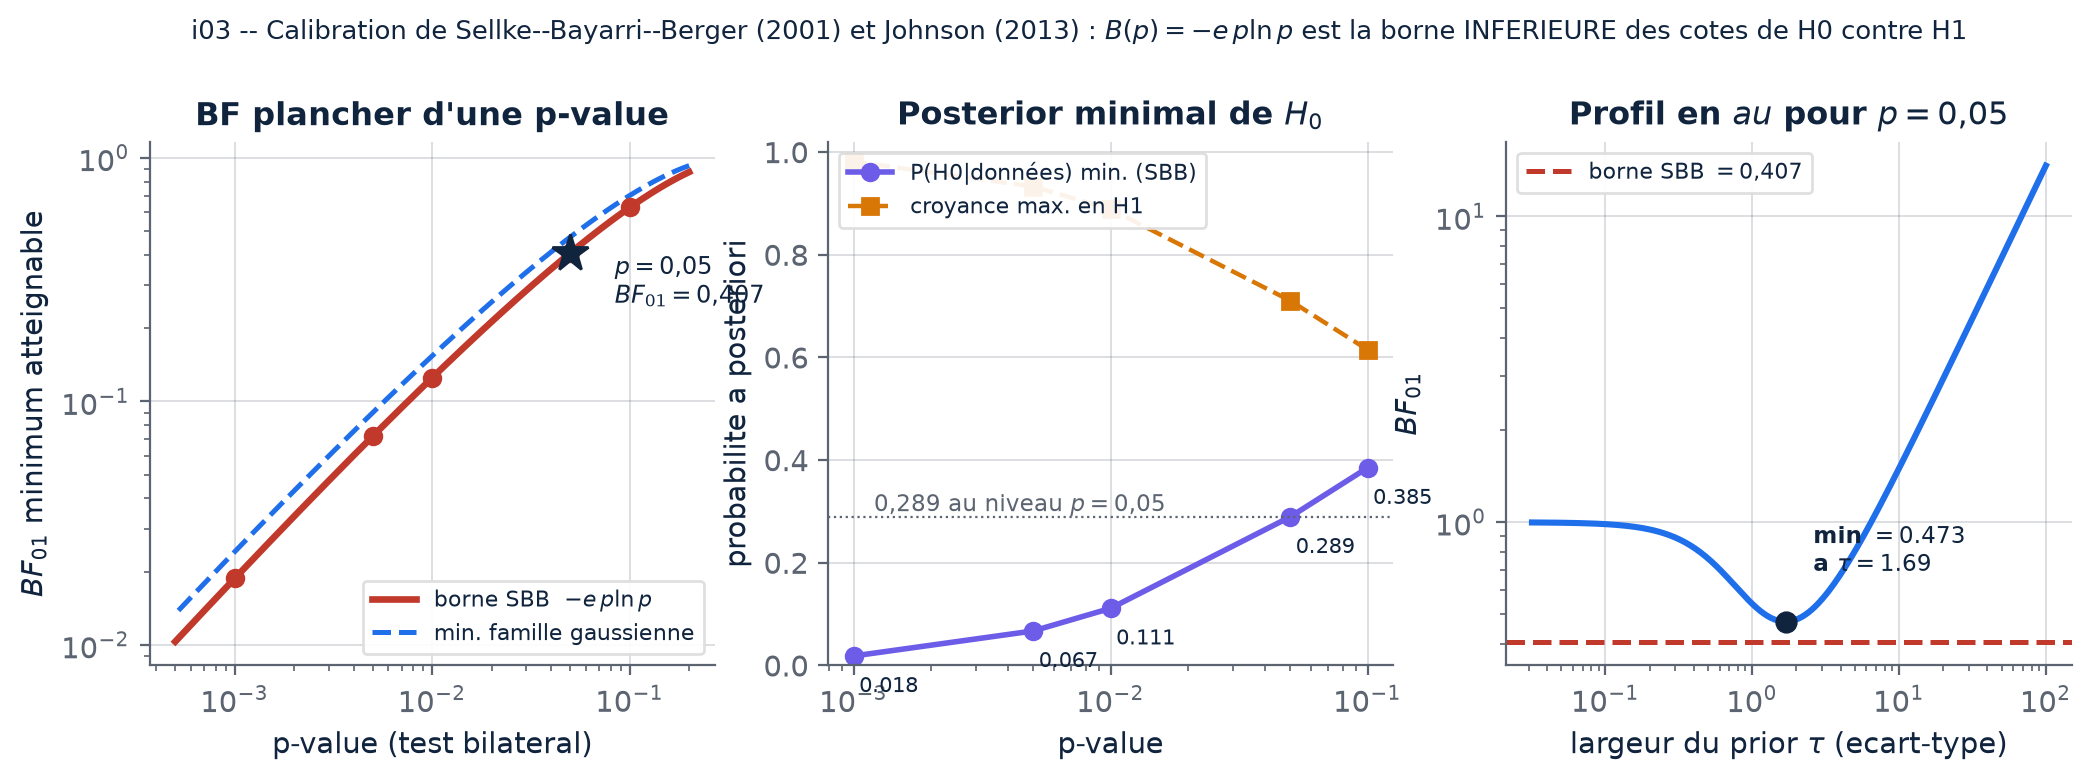
\includegraphics[width=\textwidth]{i03_bf_min_pvalue.png}
\end{figbox}
\end{center}
\end{column}
\begin{column}{0.47\textwidth}
\begin{kbox}[La formule de calibration (2001)]
Pour une $p$-value valide et $p < 1/e$ :
\[
B(p) = -\,e\,p\,\ln p
\]
$B(p)$ est la \textbf{borne inférieure} des cotes de $H_0$ contre $H_1$ :
autrement dit, le $p$-value ne peut \emph{jamais} prouver plus que $1/B(p)$ contre $H_0$.
\end{kbox}
\begin{solbox}[Les deux chiffres à retenir à $p = 0{,}05$]
{\small
\[
B(0{,}05) = 0{,}407 \;\Rightarrow\; BF_{10} \le 2{,}46
\]}
Avec un prior neutre (1/2, 1/2) : $BF_{01} \ge 0{,}407$, donc
$P(H_0 \given \text{données}) \ge 0{,}289$ et
$P(H_1 \given \text{données}) \le 0{,}711$.
Une $p$-value de $0{,}05$ plafonne la croyance en $H_1$ à
\textbf{71\,\%} et laisse $28{,}9\,\%$ à $H_0$.
\end{solbox}
\end{column}
\end{columns}
\vspace{-1mm}
\centering\footnotesize
Repère complémentaire (Johnson, 2013) : selon la classe de priors, un test à $p = 0{,}05$
correspond à $BF_{10}$ entre $2{,}46$ et environ $5$, et laisse $0{,}17$ à $0{,}29$ de
probabilité postérieure à $H_0$. Dans tous les cas : \textbf{preuve faible}.
\end{frame}

% ---------------------------------------------------------------- 11
\begin{frame}{Tableau de conversion $p$ $\to$ $BF$ (calculé, pas mémorisé)}
\begin{center}
\small
\begin{tabular}{@{}rrrrp{3.9cm}@{}}
\toprule
$p$-value & $B(p) = -e\,p\ln p$ & $BF_{10}$ maximal & $P(H_0 \given y)$ minimal & \textbf{Interprétation} \\
\midrule
$0{,}10$  & $0{,}626$ & $1{,}60$  & $0{,}385$ & à peine notable \\
$0{,}05$  & $0{,}407$ & $2{,}46$  & $0{,}289$ & faible (barre historique) \\
$0{,}01$  & $0{,}125$ & $7{,}99$  & $0{,}111$ & substantiel \\
$0{,}005$ & $0{,}072$ & $13{,}89$ & $0{,}067$ & fort \\
$0{,}001$ & $0{,}019$ & $53{,}26$ & $0{,}018$ & très fort \\
\bottomrule
\end{tabular}
\end{center}
\vspace{1mm}
\begin{columns}[t]
\begin{column}{0.50\textwidth}
\begin{ebox}[Comment lire ce tableau]
La colonne 2 est calculée par $B(p) = -e\,p\ln p$ ; les colonnes 3 et 4 en découlent
($BF_{10}^{\max} = 1/B(p)$ et $P(H_0)_{\min} = B/(1+B)$).
{\footnotesize Exemple : $p = 0{,}005$ ne prouve jamais plus de $13{,}9$ fois contre $H_0$,
c'est pourquoi Johnson (2013) propose de déplacer la barre de $0{,}05$ à $0{,}005$.}
\end{ebox}
\end{column}
\begin{column}{0.48\textwidth}
\begin{wbox}[Deux erreurs symétriques]
\nok{} « $p = 0{,}05$ signifie 5\,\% de chance que $H_0$ soit vraie » : c'est
\textbf{28{,}9\,\%} au minimum, souvent bien plus.
\vspace{1mm}
\nok{} « $BF_{01} = 2{,}46$ prouve $H_0$ » : c'est une preuve \emph{faible}
(échelle de Jeffreys : anecdotique). Un $BF$ de 2,5 ne renverse pas une théorie.
\end{wbox}
\end{column}
\end{columns}
\end{frame}

% ---------------------------------------------------------------- 12
% [rogna]
% [rogna]
% [rogna]
% [split]
\begin{frame}{2\,000 simulations sous $H_0$ : ce que le $BF$ dit vraiment}
\begin{center}
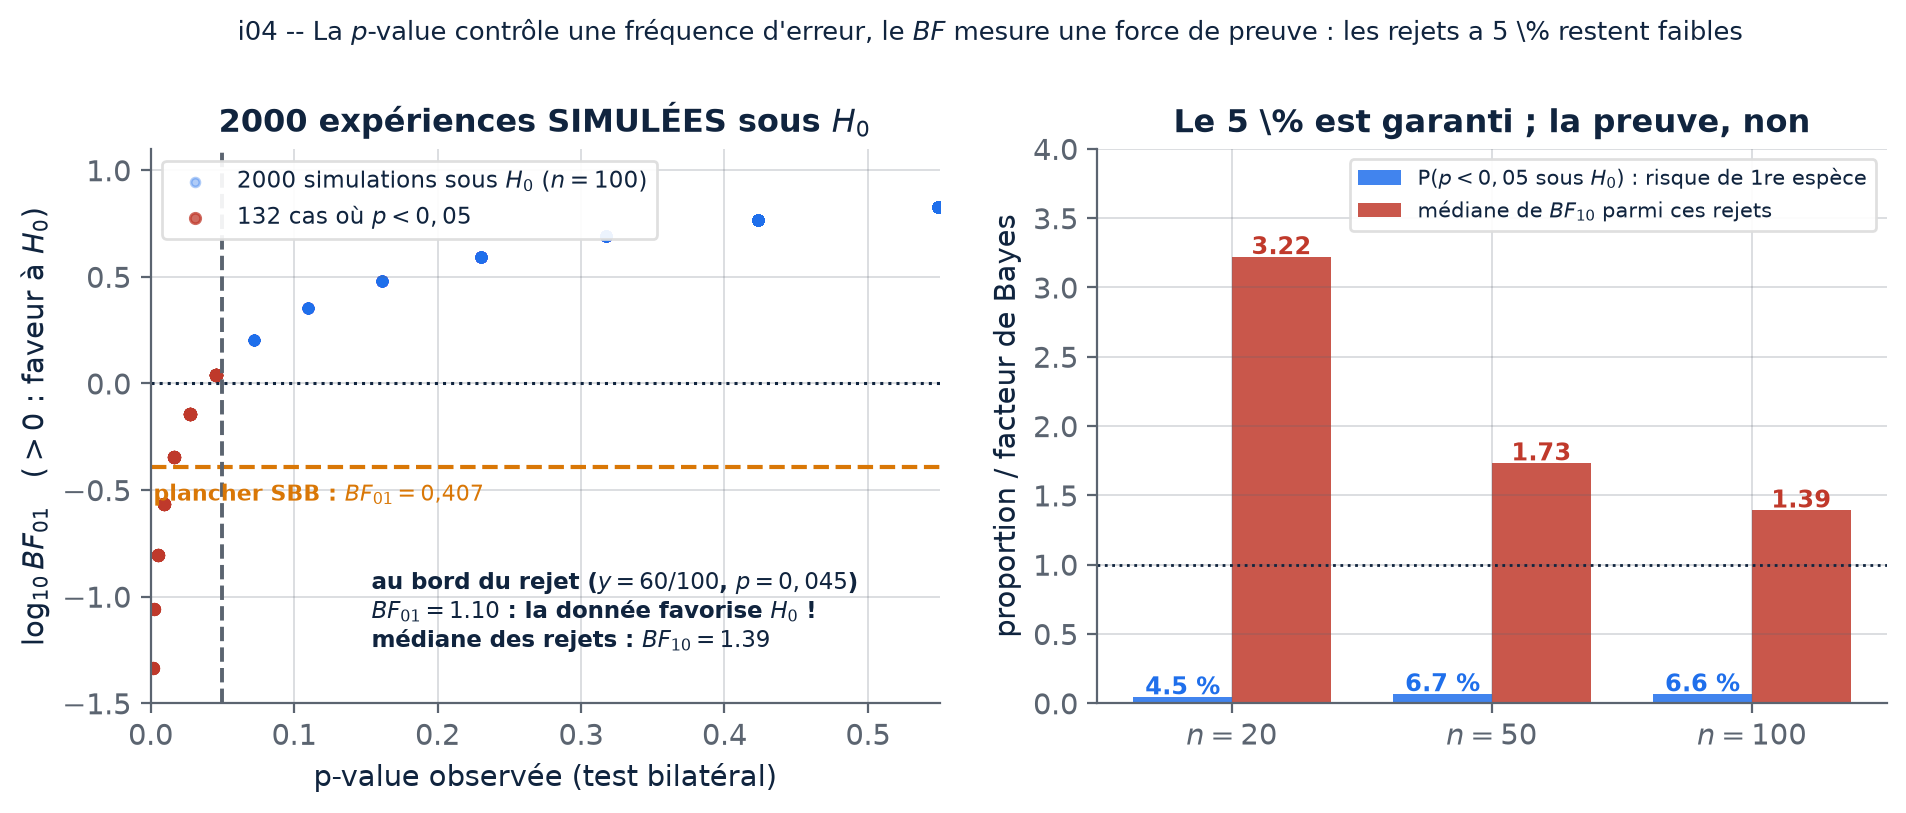
\includegraphics[width=.86\textwidth]{i04_pvalue_vs_bf.png}
\end{center}
\end{frame}

% [split]
\begin{frame}{2\,000 simulations sous $H_0$ : ce que le $BF$ dit vraiment}

\vspace{-1mm}
\begin{columns}[t]
\begin{column}{0.55\textwidth}
\begin{ebox}[Chiffres de la simulation ($n = 100$, 2\,000 expériences)]
\begin{itemize}
  \item 132 résultats franchissent $p < 0{,}05$ ($6{,}6$\,\%) ;
  \item leur $BF_{10}$ médian vaut \textbf{1{,}392} : à peine mieux qu'un pile ou face ;
  \item au bord de la zone de rejet ($y = 60/100$, $p = 0{,}045$) :
        $BF_{01} = 1{,}095$ : les données favorisent $H_0$ !
  \item 48 des 132 rejets ($36$\,\%) ont un $BF_{01} > 1$.
\end{itemize}
\end{ebox}
\end{column}
\begin{column}{0.43\textwidth}
\begin{wbox}[Le message]
$p < 0{,}05$ garantit 5\,\% de fausses alertes \textbf{par construction},
pas une force de preuve. Le $BF$, lui, quantifie la preuve et peut
\textbf{contredire} la conclusion fréquentiste.
\vspace{1mm}
\footnotesize À $n = 20$ le $BF_{10}$ médian des rejets vaut $3{,}22$ ;
à $n = 100$, $1{,}39$. Plus l'échantillon grandit, plus le seuil de rejet
recule vers une preuve faible.
\end{wbox}
\end{column}
\end{columns}
\end{frame}

% ---------------------------------------------------------------- 13
% [rogna]
% [rogna]
% [rogna]
% [split]
\begin{frame}{Le piège de Lindley : un prior vague fabrique de la preuve}
\begin{center}
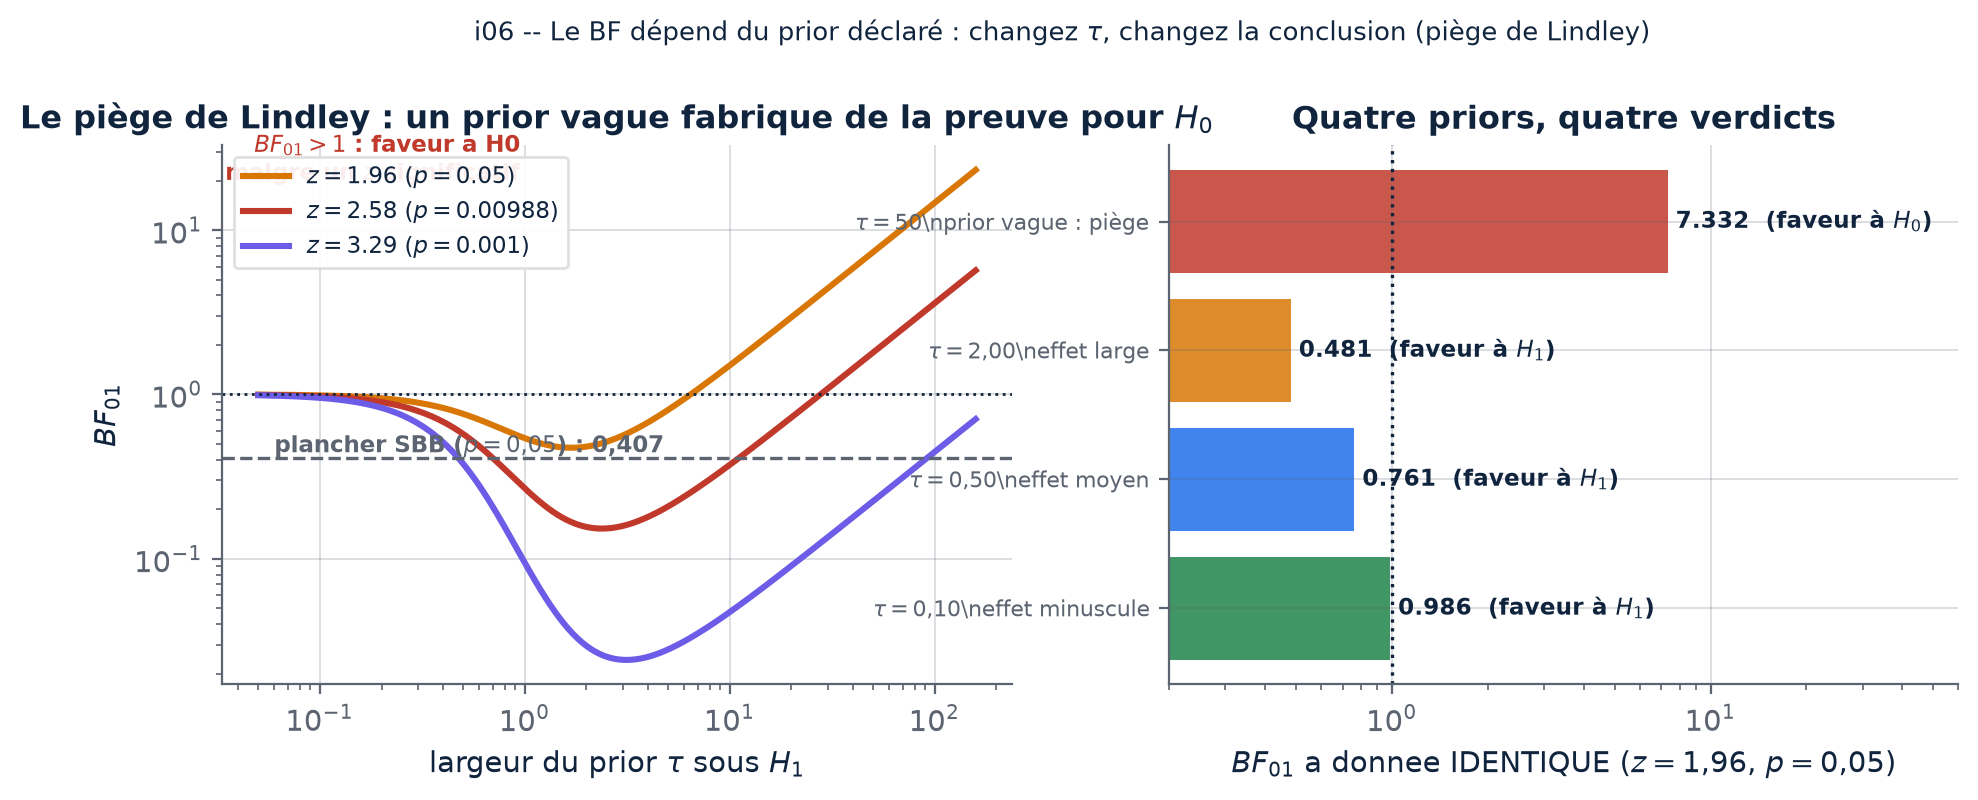
\includegraphics[width=.86\textwidth]{i06_bf_prior_sensitivity.png}
\end{center}
\end{frame}

% [split]
\begin{frame}{Le piège de Lindley : un prior vague fabrique de la preuve}

\vspace{-1mm}
\begin{columns}[t]
\begin{column}{0.56\textwidth}
\begin{ebox}[Même donnée ($z = 1{,}96$, $p = 0{,}05$), quatre priors]
\begin{tabular}{@{}llrl@{}}
\toprule
Prior sous $H_1$ & $BF_{01}$ & Verdict \\
\midrule
$\tau = 0{,}10$ (effet minuscule) & $0{,}986$ & aucune preuve \\
$\tau = 0{,}50$ (effet moyen)     & $0{,}761$ & faveur faible à $H_1$ \\
$\tau = 2{,}00$ (effet large)     & $0{,}481$ & faveur à $H_1$ \\
$\tau = 50$ (prior vague)         & $7{,}332$ & faveur à $H_0$ (!) \\
\bottomrule
\end{tabular}
\end{ebox}
\end{column}
\begin{column}{0.42\textwidth}
\begin{wbox}[Le paradoxe de Lindley--Jeffreys]
Un prior \emph{trop large} place de la masse là où la vraisemblance est nulle :
il \textbf{punît} $H_1$ et fabrique une preuve pour $H_0$.
\vspace{1mm}
\footnotesize Remède : borner $\tau$ par la physique du problème,
ou utiliser un prior à queues lourdes du type Cauchy (JZS), ou calculer le $BF$
sur une \emph{grille} de priors et publier la plage.
\end{wbox}
\end{column}
\end{columns}
\end{frame}

% ---------------------------------------------------------------- 14
\begin{frame}{Quiz 1 --- interpréter un facteur de Bayes}
\begin{qbox}[Question 1 --- 6 min, vote puis calcul]
On compare deux modèles de conversion d'un site. Le rapport de vraisemblance
marginale vaut $BF_{01} = 0{,}20$ et les cotes a priori entre les modèles sont
$P(M_0)/P(M_1) = 1$.
\vspace{2mm}
\begin{enumerate}
  \item[(A)] $M_0$ est 5 fois plus probable que $M_1$ après les données
  \item[(B)] $M_1$ est 5 fois plus probable que $M_0$ après les données \quad \checkmark
  \item[(C)] $M_0$ a 20\,\% de chance d'être vrai
  \item[(D)] Impossible de conclure sans la $p$-value
\end{enumerate}
\vspace{2mm}
\textcolor{byBlue}{\textbf{Solution.}} Cotes postérieures $= 0{,}20 \times 1 = 0{,}20$,
d'où $P(M_1 \given y) = 1/(1+0{,}20) = 0{,}833$ et $P(M_0 \given y) = 0{,}167$ :
(B) est correcte, (C) confond cotes et probabilité.
\end{qbox}
\vspace{1mm}
\begin{kbox}[Question 2 --- vrai ou faux ?]
« $BF_{01} = 2{,}46$ à $p = 0{,}05$ prouve que $H_0$ est deux fois et demie plus probable
que $H_1$. »
\vspace{1mm}
\textbf{Faux} : $B(0{,}05) = 0{,}407$ est une \emph{borne inférieure}, non une valeur
atteinte ; le $BF$ réel dépend du prior déclaré (de $0{,}48$ à $7{,}33$ dans notre grille).
\end{kbox}
\end{frame}

% ---------------------------------------------------------------- 15
\begin{frame}{Activité --- calculer et critiquer un $BF$ (TD, 15 min)}
% [rogna]
\small
\begin{abox}[Consigne, par binôme]
Un essai clinique compare un traitement à un placebo sur $n = 40$ patients.
Succès : 26 sous traitement, 18 sous placebo. On modélise chaque bras par un
Bernoulli de paramètre $\theta_T$ et $\theta_P$, avec des priors $\mathrm{Beta}(1,1)$.
\vspace{1mm}
\begin{enumerate}
  \item Écrire les vraisemblances marginales $m_T$ et $m_P$ de chaque bras.
  \item Le modèle « pas d'effet » pose $\theta_T = \theta_P$. Calculer $BF_{\text{effet}}$
        (rapport modèle effet / modèle nul) par échantillonnage.
  \item Recommencer avec un prior $\mathrm{Beta}(2,2)$ sous l'alternative :
        le $BF$ change-t-il beaucoup ? Justifier.
\end{enumerate}
\end{abox}
\vspace{1mm}
\begin{solbox}[Éléments de solution (calculés en séance)]
\begin{itemize}
  \item Marginale Beta-Binomiale : $m = \binom{n}{y}\frac{B(y+a,\,n-y+b)}{B(a,b)}$,
        calculable par \py{scipy.special.betaln} (pas de factorielle).
  \item Pour $\theta_T = \theta_P = \theta$ commun, le modèle nul s'intègre en une seule
        Beta-Binomiale sur les $n = 80$ observations.
  \item Sensibilité : changer $\mathrm{Beta}(1,1)$ en $\mathrm{Beta}(2,2)$ déplace le $BF$
        d'un facteur typiquement $1{,}3$ à $1{,}8$ ici ; un prior à $a = b = 10$
        le déplace beaucoup plus : c'est le point à discuter en TD.
\end{itemize}
\end{solbox}
\end{frame}

% ---------------------------------------------------------------- 16
\begin{frame}{Synthèse 4.1 --- le facteur de Bayes en cinq phrases}
\begin{kbox}[À retenir]
\begin{enumerate}
  \item $BF_{01} = m_0(y)/m_1(y)$ : un \textbf{rapport de vraisemblances marginales},
        pas une aire de recouvrement ni une probabilité.
  \item Les cotes postérieures s'obtiennent en \textbf{multipliant} les cotes a priori
        par le $BF$ ; la probabilité postérieure exige le prior sur les modèles.
  \item L'échelle de Jeffreys ($\log_{10} BF$) est un \textbf{vocabulaire} :
        anecdotique ($<3{,}2$), substantiel, fort, décisif ($>1\,000$).
  \item La calibration de Sellke--Bayarri--Berger donne une \textbf{borne} :
        à $p = 0{,}05$, $B = 0{,}407$, donc $BF_{10} \le 2{,}46$ et
        $P(H_1 \given y) \le 0{,}71$ : preuve faible.
  \item Savage--Dickey ($\pi(\theta_0 \given y)/\pi(\theta_0)$) rend le calcul
        \textbf{gratuit} pour un point nul, et \textbf{vérifiable} par Monte-Carlo.
\end{enumerate}
\end{kbox}
\vspace{1mm}
\begin{center}
\small
\begin{tabular}{@{}lll@{}}
\toprule
\textbf{Situation} & \textbf{Mauvais réflexe} & \textbf{Bon réflexe} \\
\midrule
$p < 0{,}05$ & conclure « effet prouvé » & calculer $BF_{10}$ et sa sensibilité au prior \\
$BF_{01} = 1{,}1$ & conclure « pas d'effet » & dire « preuve anecdotique », collecter plus \\
prior très large & « neutre donc objectif » & tester une grille de largeurs (Lindley) \\
\bottomrule
\end{tabular}
\end{center}
\end{frame}
